\documentclass[a4paper,14pt]{extarticle}

\usepackage[utf8]{inputenc}
\usepackage[T2A]{fontenc}
\usepackage[english, russian]{babel}

\usepackage[mode=buildnew]{standalone}
\usepackage{setspace}


% Различные пакеты
\usepackage{
	amssymb, amsfonts, amsmath, amsthm, physics,
	cancel, indentfirst,makecell,multirow, 
	graphicx, tikz, mathtools, float, setspace,caption,subcaption
} 

\usepackage{mathtools}

% Эта опция включает нумерацию только у тех формул,
% на которые есть ссылка в документе
\mathtoolsset{showonlyrefs=true} 

 % Цвета для гиперссылок
\definecolor{linkcolor}{HTML}{000000} % цвет ссылок
\definecolor{urlcolor}{HTML}{799B03} % цвет гиперссылок
 
\usepackage{xcolor}
\usepackage[
    unicode, 
    colorlinks, 
    urlcolor=urlcolor, 
    linkcolor=linkcolor,
    citecolor=linkcolor
]{hyperref}

% Увеличенный межстрочный интервал, французские пробелы
\linespread{1.2} 
\frenchspacing 

%%%%%%%%%%%%%%%%%%%%%%%%%%%%%%
%  Пользовательские команды  %
%%%%%%%%%%%%%%%%%%%%%%%%%%%%%%


\makeatletter
    \newcommand{\fftStar}[1]{\mathfrak{F}^*\qty[#1]}
    \newcommand{\fftNoStar}[1]{\mathfrak{F}\qty[#1]}
    \newcommand{\fft}{
                 \@ifstar
                 \fftStar%
                 \fftNoStar%
    }
\makeatother

\makeatletter
    \newcommand{\ifftNoStar}[1]{\mathfrak{F}^{-1}\qty[#1]}
    \newcommand{\ifftStar}[1]{\qty(\mathfrak{F}^{-1}\qty[#1])^*}
    \newcommand{\ifft}{
                 \@ifstar
                 \ifftStar%
                 \ifftNoStar%
    }
\makeatother

\newcommand{\mean}[1]{\langle#1\rangle}
\newcommand\ct[1]{\text{\rmfamily\upshape #1}}
\newcommand*{\const}{\ct{const}}
\renewcommand{\phi}{\varphi}
\renewcommand{\epsilon}{\varepsilon}
%\renewcommand{\sigma}{\varsigma}


\captionsetup{subrefformat=parens}

\usepackage{array}
\usepackage{pstool}


% Диагональная ячейка в таблице ( типа |a/b|)
\newcolumntype{x}[1]{>{\centering\arraybackslash}p{#1}}
\newcommand\diag[4]{%
  \multicolumn{1}{p{#2}|}{\hskip-\tabcolsep
  $\vcenter{\begin{tikzpicture}[baseline=0,anchor=south west,inner sep=#1]
      \path[use as bounding box] (0,0) rectangle (#2+2\tabcolsep,\baselineskip);
      \node[minimum width={#2+2\tabcolsep},minimum height=\baselineskip+\extrarowheight] (box) {};
      \draw (box.north west) -- (box.south east);
      \draw (box.south west) -- (box.north west);
      \node[anchor=south west] at (box.south west) {\footnotesize#3};
      \node[anchor=north east] at (box.north east) {\footnotesize#4};
 \end{tikzpicture}}$\hskip-\tabcolsep}}

%%%%%%%%%%%%%%%%%%%%%%%%%%%%%
%  Геометрия и колонтитулы  %
%%%%%%%%%%%%%%%%%%%%%%%%%%%%%


\usepackage{geometry}
\geometry       
    {
        left            =   2cm,
        right           =   2cm,
        top             =   2.5cm,
        bottom          =   2.5cm,
        bindingoffset   =   0cm
    }

% Настройка содержания, точки после нумераций
\usepackage{tocloft}
\addto\captionsrussian{\renewcommand{\contentsname}{Оглавление}}
\renewcommand{\cftsecleader}{
	\cftdotfill{\cftdotsep}}
% \renewcommand{\thesection}{
	% \arabic{section}.}
% \renewcommand{\thesubsection}{
	% \arabic{section}.\arabic{subsection}.}
% \renewcommand{\thesubsubsection}{
	% \arabic{section}.\arabic{subsection}.\arabic{subsubsection}.}     
\usepackage[explicit]{titlesec}

% Колонтитулы
%\usepackage{fancyhdr} 
	%\pagestyle{plain} 
	%\fancyhead{} 
	%\fancyhead[R]{} 
	%\fancyhead[L]{} 
	%\fancyfoot{} 
	%\fancyfoot[C]{\thepage} 

\NewDocumentCommand{\codeword}{v}{%
\texttt{\textcolor{gray}{#1}}%
}
\usepackage{listings,multicol}
\usepackage{courier}
\definecolor{mygreen}{rgb}{0,0.6,0}
\definecolor{mygray}{rgb}{0.5,0.5,0.5}
\definecolor{mymauve}{rgb}{0.58,0,0.82}
\newcommand{\python}[1]{\lstinline[basicstyle=\normalsize\ttfamily]{#1}}

\lstset{ 
  backgroundcolor=\color{white},   % choose the background color; you must add \usepackage{color} or \usepackage{xcolor}; should come as last argument
  basicstyle=\footnotesize\ttfamily,        % the size of the fonts that are used for the code
  breakatwhitespace=false,         % sets if automatic breaks should only happen at whitespace
  breaklines=true,                 % sets automatic line breaking
  captionpos=b,                    % sets the caption-position to bottom
  commentstyle=\color{mygreen},    % comment style
  deletekeywords={...},            % if you want to delete keywords from the given language
  escapeinside={\%*}{*)},          % if you want to add LaTeX within your code
  extendedchars=true,              % lets you use non-ASCII characters; for 8-bits encodings only, does not work with UTF-8
  firstnumber=1,                % start line enumeration with line 1000
  frame=single,	                   % adds a frame around the code
  keepspaces=true,                 % keeps spaces in text, useful for keeping indentation of code (possibly needs columns=flexible)
  keywordstyle=\color{blue},       % keyword style
  language=Python,                 % the language of the code
  morekeywords={*,...},            % if you want to add more keywords to the set
  numbers=left,                    % where to put the line-numbers; possible values are (none, left, right)
  numbersep=15pt,                   % how far the line-numbers are from the code
  numberstyle=\tiny\color{mygray}, % the style that is used for the line-numbers
  rulecolor=\color{black},         % if not set, the frame-color may be changed on line-breaks within not-black text (e.g. comments (green here))
  showspaces=false,                % show spaces everywhere adding particular underscores; it overrides 'showstringspaces'
  showstringspaces=false,          % underline spaces within strings only
  showtabs=false,                  % show tabs within strings adding particular underscores
  stepnumber=1,                    % the step between two line-numbers. If it's 1, each line will be numbered
  stringstyle=\color{mymauve},     % string literal style
  tabsize=2,	                   % sets default tabsize to 2 spaces
  %title=\lstname,                   % show the filename of files included with \lstinputlisting; also try caption instead of title
  frame=none,
  %multicols=1,
  columns=fullflexible,
  extendedchars=\true,
  escapechar=!,
}




\title{Компьютерные технологии}
\author{Карусевич А. А.}
\date{}



\begin{document}
\maketitle

\paragraph{Задание 11} Создайте модель процесса остывания стеклянного стакана с горячим кофе при 
комнатных условиях. Постройте графики изменения температуры с учетом теплопроводности, 
конвекции и испарения, а также оцените точность интегрирования в зависимости от схемы 
интегрирования и величины шага интегрирования.


\section{Алгоритм решения}
Для моделирования процесса остывания стакана с кофе необходимо учесть несколько эффектов. Во-первых, теплопроводность. 

\paragraph{Учет теплопроводности} Теплопроводность описывается уравнением
теплопроводности (Heat Equation) и в общем виде выглядит следующим образом:
\begin{equation}
	\frac{\partial u}{\partial t} = a^2 \Delta u + f(r,t),
\end{equation}
где $u(x,y,t)$ - температура в пространстве и времени, $a^2$ —  коэффициент температуропроводности, $\Delta$ — оператор Лапласа и $f(r,t)$ — функция тепловых источников. 
В нашем случае кофе наливается горячим, а после остывает при комнатной
температуре, где источники отсутствуют, поэтому $f = 0$.

Чтобы описать систему кофе-стакан-воздух, введем зависимость коэффициента температуропроводности $a^2$ от координат. Соответственно в тех местах,
где расположен кофе, будет значение температуропроводности кофе, где стекло - там температуропроводность стекла и т.д.


Рассматривать задачу будем в двух измерениях X, Y, поскольку при использовании цилиндрической системы координат от
угла ничего не будет зависеть.
В двумерной декартовой системе координат оператор Лапласа запишется как
\begin{equation}
	\Delta u = \frac{\partial^2 u}{\partial x^2} + \frac{\partial^2 u}{\partial
    y^2}.
\end{equation}
Для численного расчета Лапласиана будем применять метод конечных разностей, например для частной производной по $x$:

\begin{equation}
	\frac{\partial^2 u(x_i,t)}{\partial x^2} = \frac{u(x_{i+1},t) -2 u(x_{i},t) + u(x_{i-1},t)}{\Delta x^2},
\end{equation}
где $x_i$ - принадлежит предварительно распределенной координатной сетке с заданным шагом.

\paragraph{Учет конвекции} Чтобы учесть конвекционную передачу тепла от жидкости стенке, воспользуемся законом 
Ньютона — Рихмана, описывающего теплопередачу от жидкости телу. Запишем в следующей форме:
\begin{equation}
	\frac{\partial u}{\partial n} = \frac{\alpha}{\lambda}(u_s - u),
\end{equation}
где $\frac{\partial u}{\partial n}$ - производная по нормали к поверхности тела на границе тело-жидкость, т.е. стенки стакана, $u_s$ - 
температура поверхности, $\alpha$ - коэффициент теплоотдачи, $\lambda$ - коэффициент теплопроводности.

В таком виде данный закон выступает граничным условием третьего рода для уравнения теплопроводности, описанного выше.

\paragraph{Учет испарения} В общем случае учет испарения является достаточно трудоемкой задачей. В данной работе охлаждение жидкости засчет
испарения будет учитываться в зависимости от скорости испарения массы жидкости, а также удельной теплоты испарения, откуда будет находится изменение температуры.

Скорость испарения $W$ (кг/ч) описывается как
\begin{equation}
	W = S (b + 0.0174 \cdot V) P_V(T) (1 - \frac{h}{100}),
\end{equation}
где $S$ - площадь испаряемой жидкости (м$^2$), $b$ - фактор скорости подвижности окружающего воздуха, $V$ - скорость воздуха на поверхности испаряемой жидкости,
$P_V(T)$ - давление насыщенного пара, зависящее от температуры, $h$ - влажность воздуха в процентах.

Зная массу испаряемой жидкости, а также удельную теплоту испарения $L \simeq 2260 $ кДж/кг, можно найти теплоту, потраченную жидкостью на испарение,
а значит и падение температуры в верхнем слое.


\section{Результаты моделирования}
Моделирование системы производится на языке Python.
Используется библиотека SciPy, а также встроенный для решения дифференциальных уравнений метод \text{integrate.solve\_ivp}.
В данном методе используется алгоритм Рунге-Кутты 5-го порядка, а шаг интегрирования выбирается так,
чтобы ошибка не превышала наперед заданного значения относительной $\varepsilon_r \leq 10^{-3}$ и абсолютной
ошибок $\varepsilon_a \leq 10^{-6}$ интегрирования.
Исходный код программы приведен в листинге \ref{lst:task11}.

Результаты моделирования приведены на рисунках
\ref{fig:init}, \ref{fig:10}, \ref{fig:30}, \ref{fig:120}, \ref{fig:600}, \ref{fig:temp}.

Кофе имеет изначальную температуру 350 К, а стекло и воздух вокруг 300 К.
Изначальное распределение температуры приведено на рис. \ref{fig:init}. На рисунках \ref{fig:10}, \ref{fig:30}, \ref{fig:120}, \ref{fig:600} показаны распределения 
температуры в разные моменты времени - 10, 30, 120 секунд с начала моделирования

На рис. \ref{fig:temp} приведена зависимость температуры верхней части кофе от времени.

\begin{figure}[H]
	\center
	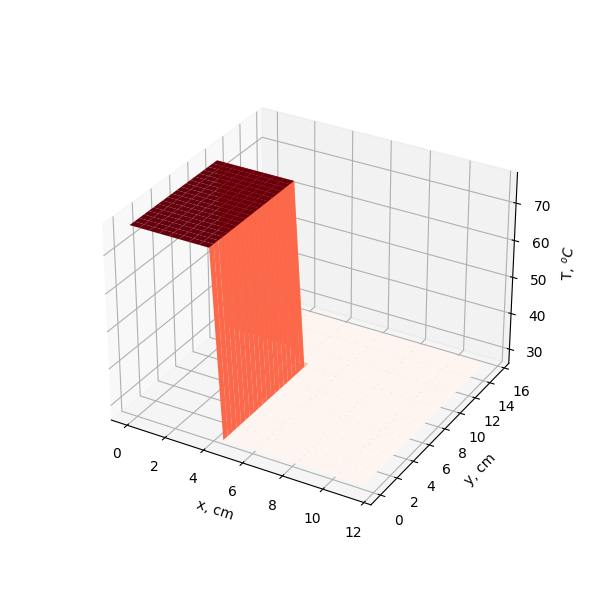
\includegraphics[width=.6\linewidth]{imgs_11/init.png}
	\caption{Начальное распределение температуры. До $x=4$ см расположено кофе, далее до $x=5$ см стеклянный стакан.
	Далее пространство заполнено воздухом}
	\label{fig:init}
\end{figure}
\begin{figure}[H]
	\center
	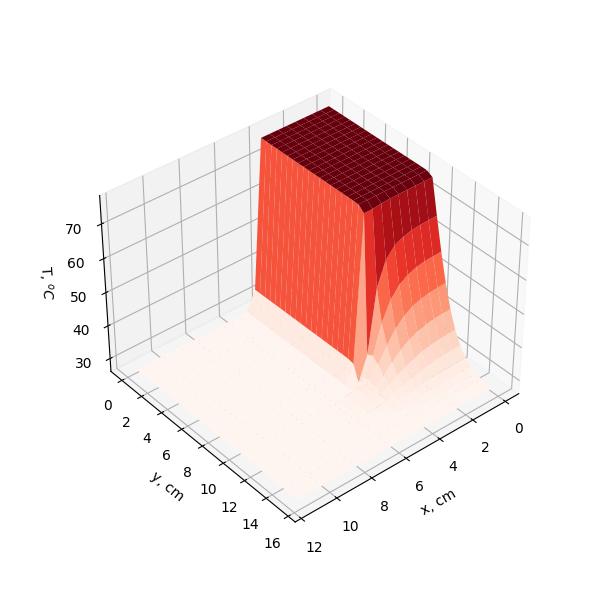
\includegraphics[width=.6\linewidth]{imgs_11/10s.png}
	\caption{Распределение температуры в $t=10$с}
	\label{fig:10}
\end{figure}
\begin{figure}[H]
	\center
	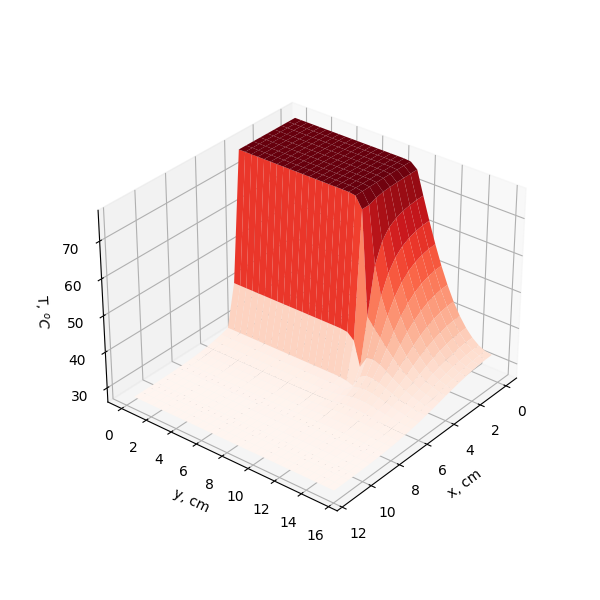
\includegraphics[width=.6\linewidth]{imgs_11/30s.png}
	\caption{Распределение температуры в $t=30$с}
	\label{fig:30}
\end{figure}
\begin{figure}[H]
	\center
	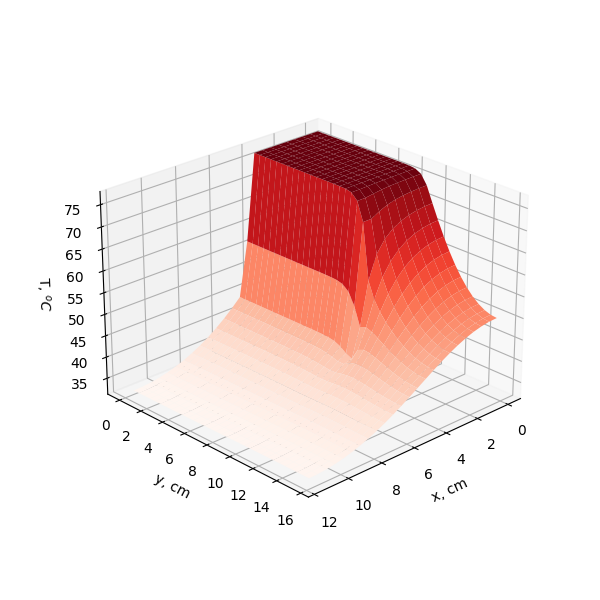
\includegraphics[width=.6\linewidth]{imgs_11/120s.png}
	\caption{Распределение температуры в $t=120$с}
	\label{fig:120}
\end{figure}
\begin{figure}[H]
	\center
	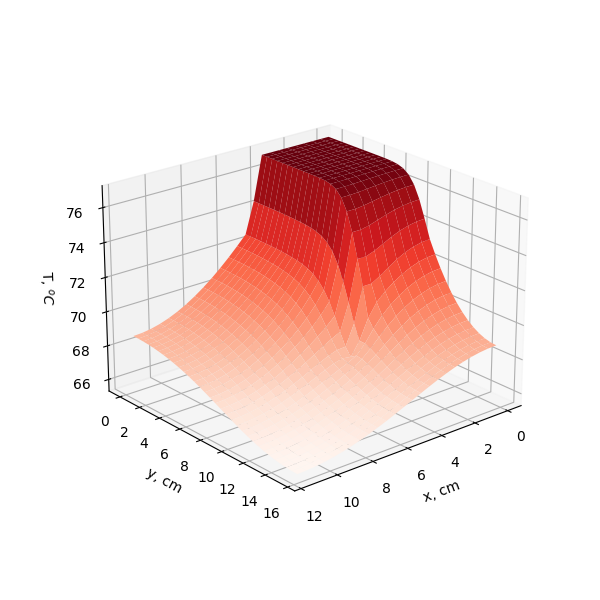
\includegraphics[width=.6\linewidth]{imgs_11/600s.png}
	\caption{Распределение температуры в $t=600$с}
	\label{fig:600}
\end{figure}

\begin{figure}[H]
	\center
	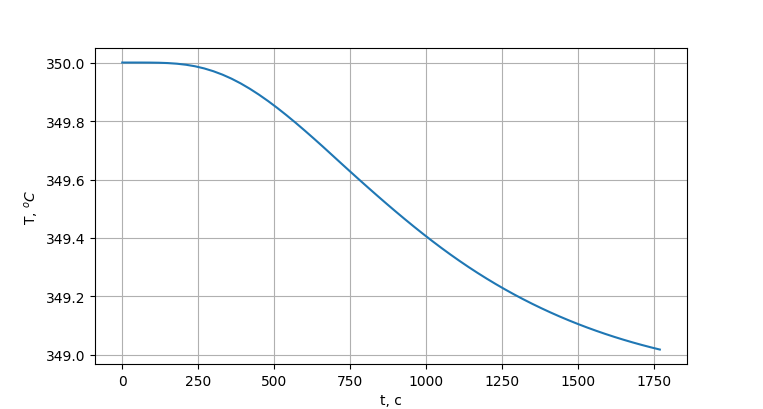
\includegraphics[width=.6\linewidth]{imgs_11/temp.png}
	\caption{Зависимость температуры в верхней части стакана кофе от времени ($x=2 , y= 0.97$ см).}
	\label{fig:temp}
\end{figure}

\newpage
\section{Исходный код}
\lstinputlisting[label={lst:task11}, caption={Исходный код задания}]{task_11.py}


\end{document}
